\documentclass[8pt]{beamer}
%\usepackage[french]{babel}
\usepackage[english]{babel}
%\usepackage[utf8]{inputenc}
%\usepackage[T1]{fontenc}
\usepackage{lmodern}
\usepackage[titlenumbered,ruled,noend,french,onelanguage,linesnumbered]{algorithm2e}
\usepackage{tikz}
\usepackage{graphicx}
%\usepackage[dvipsnames, svgnames]{xcolor}
\usepackage{array}
\usepackage{multirow}
\usepackage{caption}
\usepackage{subcaption}
\usetheme[sectionpage=none, progressbar=frametitle, numbering=fraction]{metropolis}  
%\usetheme{Antibes}
\usepackage{tabulary}

\usepackage{tcolorbox}
\definecolor{goldenrod}{RGB}{238,232,170}
%\newtcolorbox{mytitlebox}[1]{
%colback=white,
%%colbacktitle=black!10!,
%%coltitle=red!70!black,
%%colframe=red!70!black,
%coltitle=black,
%%colframe=black,
%boxrule=1pt,
%titlerule=0pt,
%arc=15pt,
%title={\strut#1}
%}


\newtcolorbox{mybox}[1][]{
colback=white,
colbacktitle=black!10!,
%coltitle=red!70!black,
%colframe=red!70!black,
coltitle=black,
colframe=black,
boxrule=1pt,
titlerule=0pt,
arc=10pt,
title={\strut\textbf{#1}}
}

%\setbeamertemplate{footline}[frame number]

\title{Image denoising with multi-layer perceptrons}
\author{ESTEVE Nathan \\ FATTOUHY Mohamed \\ NGUYEN Louis\\ VERNAY Amélie}
\date{\today}

%\titlegraphic{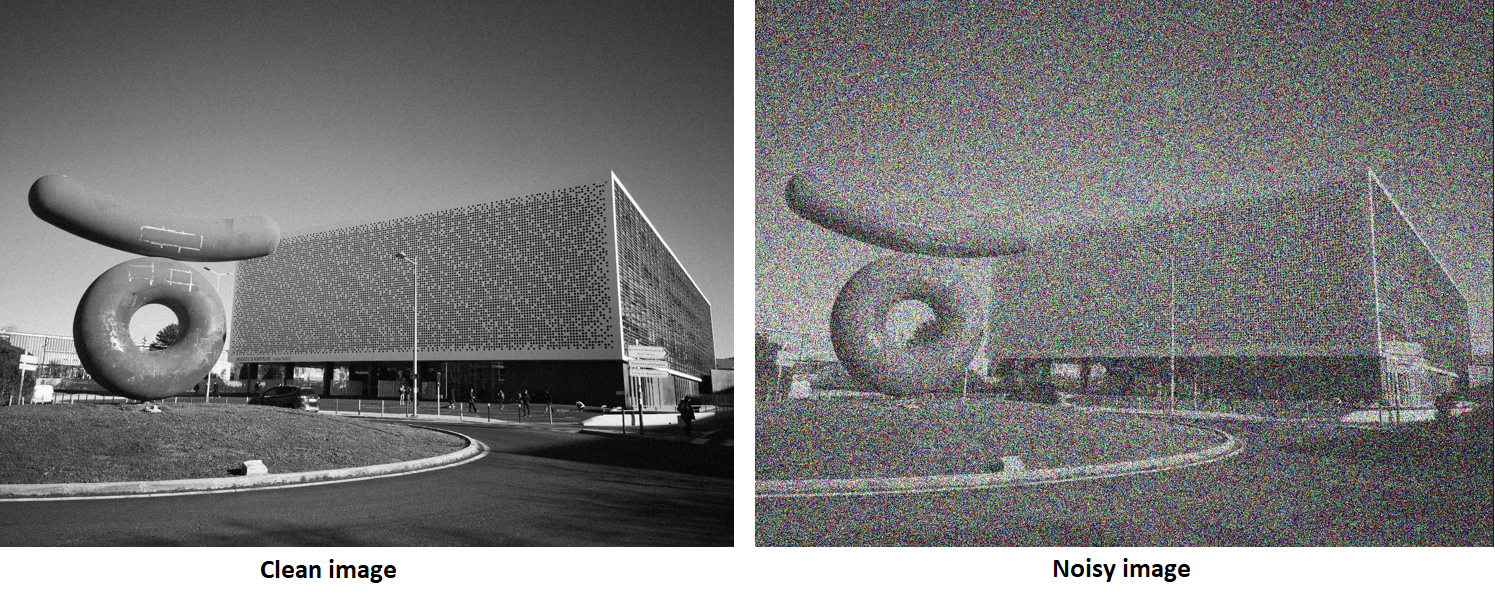
\includegraphics[scale=0.22]{../datasets/images/Image_comparaison.png}}

\titlegraphic{%
  \begin{picture}(0,0)
    \put(285,-145){\makebox(0,0)[rt]{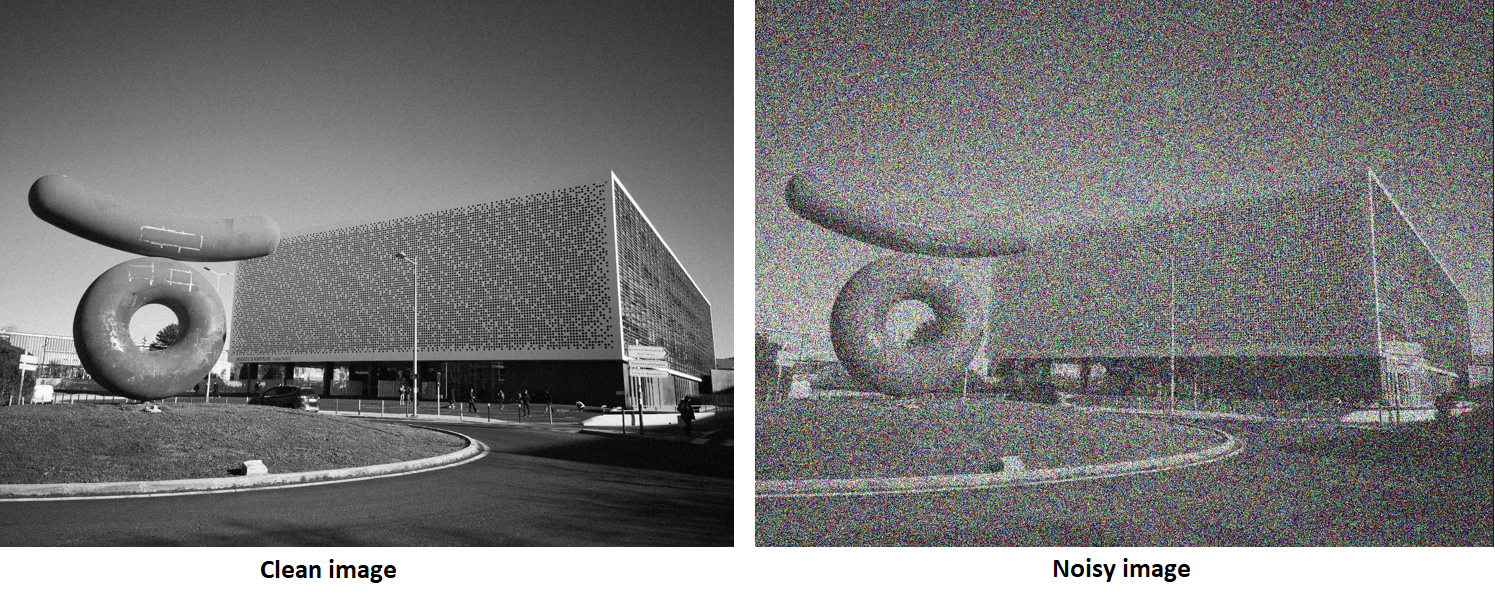
\includegraphics[scale=0.17]{../datasets/images/Image_comparaison.png}}}
  \end{picture}}


%\AtBeginSection[]
%{
%  \begin{frame}
%    \frametitle{Table of Contents}
%    \tableofcontents[currentsection]
%  \end{frame}
%}



\setbeamertemplate{navigation symbols}{}


\begin{document}


\begin{frame}[noframenumbering, plain]
\titlepage
\end{frame}

%\addtocounter{framenumber}{-1}
% \setbeamertemplate{footline}[frame number]



\begin{frame}
\frametitle{Table of content}
\tableofcontents
\end{frame}


\section{Context}

\begin{frame}{Context}
\begin{mybox}[
\emph{Image denoising with multi-layer perceptrons, part 1: comparison with existing algorithms and with bounds}, H. C. Burger, C. J. Schuler, S. Harmeling (2012)]
\end{mybox}\

%\fcolorbox{black}{white}{\emph{Image denoising with multi-layer perceptrons, part 1: comparison with existing algorithms and with bounds}, H. C. Burger, C. J. Schuler, S. Harmeling (2012)]}

% noise, denoising, patches, types de bruits

\begin{mybox}[Image denoising]
Image denoising seeks to find a clean image given only its noisy version.

\end{mybox}

\begin{mybox}[Trade-off]
Image denoising requires to denoise patches separately:

\begin{itemize}
\item very small patches lead to a function that is easily modeled, but to bad denoising results;
\item very large patches potentially lead to better denoising results, but the function might be difficult to model.
\end{itemize}

\end{mybox}


\end{frame}

\begin{frame}
    \begin{figure}[H]
        \begin{center}
            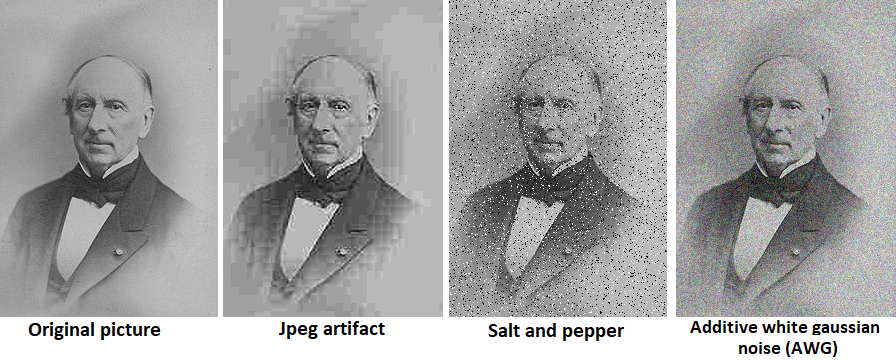
\includegraphics[scale=0.45]{../datasets/images/Allnoise.png}
            \caption{Image of Louis Augustin Cauchy with differents noises}
        \end{center}
    \end{figure}
    
\end{frame}


\section{MLP-based method}



\begin{frame}{MLP-based method}

A multi-layer perceptron is a fully connected neural network.

% ----
% Input layer neurons'number
\newcommand{\inputnum}{3} 
 
% Hidden layer neurons'number
\newcommand{\hiddennum}{5}  
 
% Output layer neurons'number
\newcommand{\outputnum}{2} 

% Input layer neurons'number
\renewcommand{\inputnum}{1} 
 
% Hidden layer neurons'number
\renewcommand{\hiddennum}{5}  
 
% Output layer neurons'number
\renewcommand{\outputnum}{1} 
% ----

% MLP tikz picture
%\begin{center}
\begin{figure}[h]% <--- '[h]' says "let figure be here"
\begin{minipage}[c]{9.5cm}
\resizebox{1\textwidth}{!}{% for a smaller picture
\begin{tikzpicture}
 
% Input Layer
\foreach \i in {1,...,\inputnum}
{
    \node[circle, minimum size = 6mm, fill = orange!40] (Input-\i) at (0,-\i) {};
}
 
% Hidden Layer
\foreach \i in {1,...,\hiddennum}
{
    \node[circle, minimum size = 6mm, fill=teal!50, yshift = (\hiddennum-\inputnum)*5 mm] (Hidden-\i) at (2.5,-\i) {};
}

% Hidden Layer
\foreach \i in {1,...,\hiddennum}
{
    \node[circle, minimum size = 6mm, fill=teal!50, yshift = (\hiddennum-\inputnum)*5 mm] (Hiddenn-\i) at (5,-\i) {};
}

% Output Layer
\foreach \i in {1,...,\outputnum}
{
    \node[circle, minimum size = 6mm, fill = brown!80, yshift = (\outputnum-\inputnum)*5 mm] (Output-\i) at (7.5,-\i) {};
}
 
% Connect neurons In-Hidden
\foreach \i in {1,...,\inputnum}
{
    \foreach \j in {1,...,\hiddennum}
    {
        \draw[->, shorten >=1pt] (Input-\i) -- (Hidden-\j);   
    }
}
 
% Connect neurons In-hidden-In-hiddenn
\foreach \i in {1,...,\hiddennum}
{
    \foreach \j in {1,...,\hiddennum}
    {
        \draw[->, shorten >=1pt] (Hidden-\i) -- (Hiddenn-\j);   
    }
}

% Connect neurons Hidden-Out
\foreach \i in {1,...,\hiddennum}
{
    \foreach \j in {1,...,\outputnum}
    {
        \draw[->, shorten >=1pt] (Hiddenn-\i) -- (Output-\j);
    }
}
 
% Inputs
\foreach \i in {1,...,\inputnum}
{            
    \draw[<-, shorten <=1pt] (Input-\i) -- ++(-1,0) node[left]{$x_{noisy}$};
}
 
% Outputs
\foreach \i in {1,...,\outputnum}
{            
    \draw[->, shorten <=1pt] (Output-\i) -- ++(1,0) node[right]{$f(x_{noisy})$};
}


\node[above] at (0, 0 |- 0,2.5) {Input layer};
\node[above] at (2.5, 0 |- 2.5,2.5) {Hidden layer 1};
\node[above] at (5, 0 |- 2.5,2.5) {Hidden layer 2};
\node[above] at (7.5, 0 |- 2.5,2.5) {Output layer};
\end{tikzpicture}
%\end{center}
}% end reducing picture size
\end{minipage}%
\end{figure}

\vspace{7pt}

$x_{noisy}$ is a noisy version of a clean patch $x$; $f(x_{noisy})$ represents an estimate of $x$.

\end{frame}


\begin{frame}
% Expliqué INPUT/OUTPUT + POIDS W + LOSS (SNR)
\begin{mybox}[Weight initialization for MLP-based method]
Weights $w$ are sampled from an uniform distribution :  \\%Weight are randomly initialize following a uniform distribution:\\
$$w \sim U\left[-\frac{\sqrt{6}}{\sqrt{n_j + n_{j+1}}}, \frac{\sqrt{6}}{\sqrt{n_j + n_{j+1}}}\right]$$

{\footnotesize $n_j$ and $n_{j+1}$ are the number of neurons in the input and output sides of the layer.}
%$n_j$ (resp. $n_{j+1}$) the number of neurons in the input (resp. output) side of the layer
\end{mybox}

\begin{mybox}[Loss function]
The loss function used is the MSE : $$MSE = \frac{1}{n} \sum_{i=1}^{n} \ (f(x_i)-x_i)^2,$$ where $x$ is a clean patch and $f(x)$ the estimation of $x$.
\end{mybox}

\begin{mybox}[Peak Signal-To-Noise Ratio (PSNR)]
PSNR = $20 \times \log_{10}\left(\dfrac{m}{\sqrt{\mathrm{MSE}}} \right)$ (dB), where $m$ is the maximum possible pixel value of a given image.
\end{mybox}
\end{frame}

\section{Results}

\begin{frame}{Results for AWG noise}
%\begin{mybox}[Definition]
%Additive white Gaussian noise (AWG) : Mimics the effect of many random processes that occur in nature. 
%%(Source: Wiki)
%\end{mybox} 

\begin{figure}[H]
    \begin{center}
        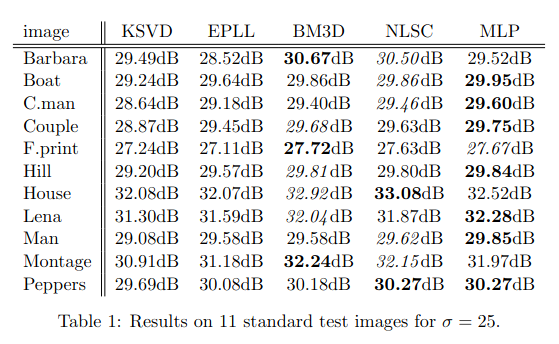
\includegraphics[scale=0.40]{../datasets/images/Table_dB.png}
        %\caption{Comparaison BM3D and MLP (AWG noise $\sigma = 25 $)}
    \end{center}
\end{figure}

\end{frame}

\begin{frame}{Results for AWG noise}
%\begin{mybox}[Definition]
%Additive white Gaussian noise (AWG) : Mimics the effect of many random processes that occur in nature. 
%%(Source: Wiki)
%\end{mybox} 

\begin{figure}[H]
    \begin{center}
        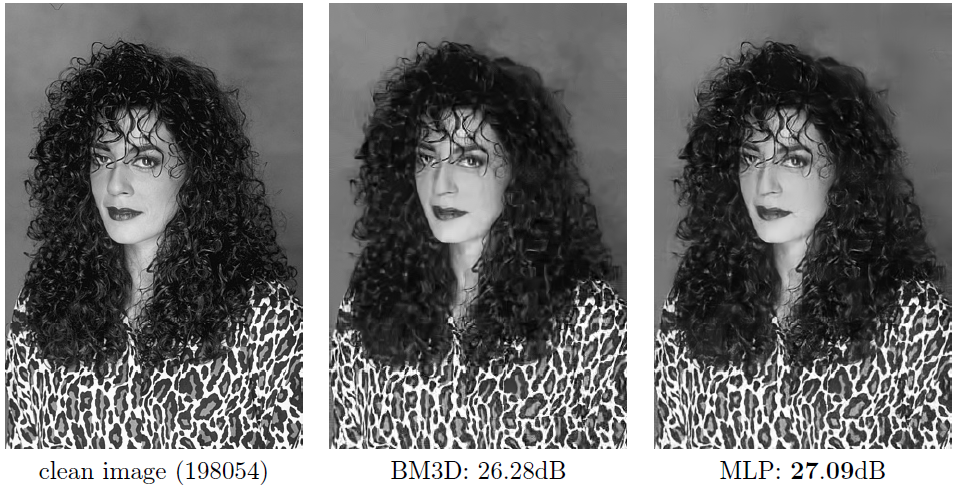
\includegraphics[scale=0.40]{../datasets/images/barbara.png}
        \caption{BM3D and MLP performances (AWG noise $\sigma = 25 $)}
    \end{center}
\end{figure}

\end{frame}

\section{Bounds}

\begin{frame}{Bounds}

\begin{mybox}[Clustering-based bounds]
There exist inherent limits on denoising quality for images with rich geometric structure.
\end{mybox}\

\begin{mybox}[Bayesian framework]
Bayesian bounds estimate how well any denoising algorithm can perform in a bayesian framework which depends on the patch size.
\end{mybox}

\end{frame}

\begin{frame}{Other types of noise}
%We begin by Strip noise, see result of denoising with BM3D and MLP.

\begin{figure}[H]
    \begin{center}
        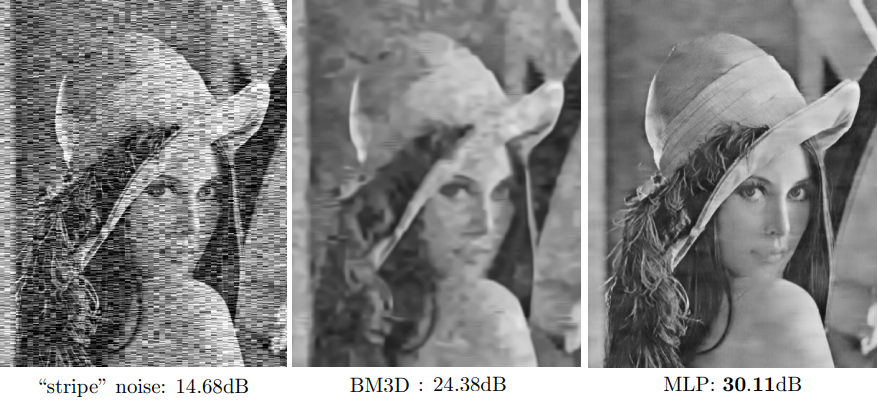
\includegraphics[scale=0.45]{../datasets/images/stripnoise.png}
        \caption{MLP and BM3D performances on strip noise}
    \end{center}
\end{figure}
\end{frame}



\begin{frame}{Other types of noise}
%For Salt and pepper noise, we compare MLP with median filtering methode. This method was the stat-of-the-art for this type of noise.
\begin{figure}[H]
    \begin{center}
        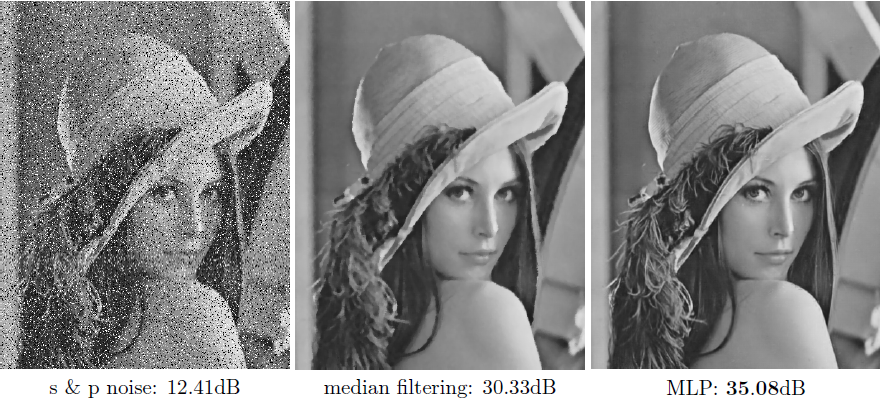
\includegraphics[scale=0.45]{../datasets/images/saltandpeppernoise.png}
        \caption{MLP and median filtering performances on salt and pepper noise}
    \end{center}
\end{figure}

\end{frame}

\begin{frame}{Other types of noise}
    %For JPEG articact, we compare MLP againt the state-of-the-art. 

    \begin{figure}[H]
        \begin{center}
            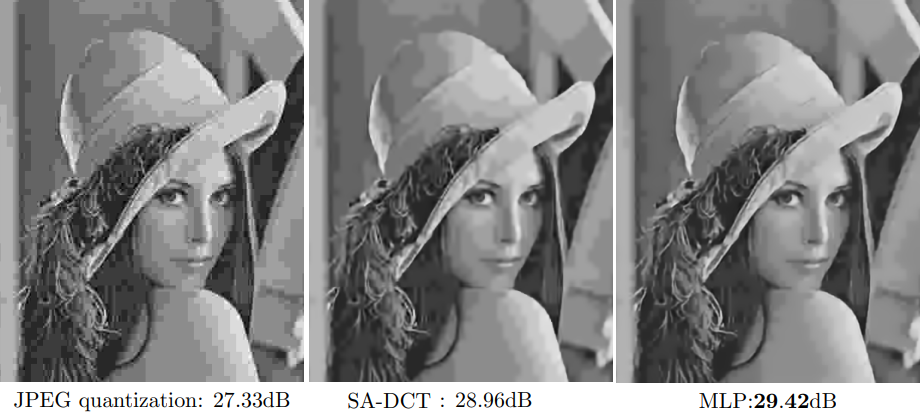
\includegraphics[scale=0.45]{../datasets/images/Jpgegnoise.png}
            \caption{MLP and median filtering performances on JPEG Artifact}
        \end{center}
    \end{figure}
    
\end{frame}

\section{Block-matching}
\begin{frame}{Block-matching}
\begin{mybox}[Block-matching]
We look for the patches most similar to a reference patch.
\end{mybox}\

\begin{mybox}[Combine MLP and block-matching]
We train MLPs that take as input a reference patch and its nearest neighbors (similar patches).
\end{mybox}\

\begin{mybox}[Results]
Block-matching MLPs provide better results on images with repeating structure than plain MLPs.

\vspace{0.5em}
However, BM3D and NLSC still provide better results on this kind of images.
\end{mybox}
\end{frame}






\section{Conclusion}

\begin{frame}{Conclusion}
%\begin{mybox}{}
%
%\end{mybox}
\begin{itemize}
	\item Excellent results BUT outperformed by BM3D and NLSC on images with a lot a regular structure.
	\item The MLP-based approach achieves excellent results, no matter the type of noise, especially with high levels of noise.
	\item The MLP-based approach shows that it is possible to significantly improve denoising quality on images with complex textures.
	\item Would it be possible to find an approach that would perform state-of-the-art results on every image ?
	
\end{itemize}

\end{frame}


\end{document}
